\documentclass[a4paper]{article}

%------------------------------------------------------------
\usepackage[a4paper, total={6in, 9in}]{geometry}
\usepackage{amsmath, amssymb}
\usepackage{booktabs}
\usepackage{caption}
\usepackage{enumitem}
\usepackage{graphicx}
\usepackage{float}
\usepackage{inconsolata}
\usepackage{listings}
\usepackage{mathtools}
\usepackage{pstricks-add}
\usepackage{siunitx}
\usepackage[most]{tcolorbox}
\usepackage{tikz, pgfplots}
\usepackage{epstopdf} %converting to PDF
\usepackage{hyperref}
\usepackage{xfrac}

\usetikzlibrary{shapes.geometric}
\usetikzlibrary{arrows}

%------------------------------------------------------------
\graphicspath{{./fig/}}
\pgfplotsset{compat=1.13}
%------------------------------------------------------------
\setlength{\parindent}{0in}

\lstdefinestyle{C++}{
	language=C++,
	basicstyle=\ttfamily,
	keywordstyle=\color{blue}\ttfamily,
	stringstyle=\color{red}\ttfamily,
	commentstyle=\color{green}\ttfamily,
	morecomment=[l][\color{magenta}]{\#},
	showstringspaces=false
}

%------------------------------------------------------------
\newtcblisting[auto counter]{sexylisting}[2][]{sharp corners, 
    fonttitle=\bfseries, colframe=gray, listing only, 
    listing options={basicstyle=\ttfamily,language=C++}, 
    title=Listing \thetcbcounter: #2, #1}

%------------------------------------------------------------
\lstset{language=C++,
        basicstyle=\ttfamily,
        keywordstyle=\color{blue}\ttfamily,
        stringstyle=\color{red}\ttfamily,
        commentstyle=\color{green}\ttfamily,
        morecomment=[l][\color{magenta}]{\#},
        showstringspaces=false
}
%------------------------------------------------------------
\tikzstyle{block} = [draw, fill=blue!20, rectangle, 
    minimum height=3em, minimum width=3em]
\tikzstyle{sum} = [draw, fill=blue!20, circle, node distance=1cm]
\tikzstyle{input} = [coordinate]
\tikzstyle{output} = [coordinate]
\tikzstyle{pinstyle} = [pin edge={to-,thin,black}]

%------------------------------------------------------------
\newlength{\arrow}
\settowidth{\arrow}{\scriptsize$1000$}
\newcommand*{\myrightarrow}[1]{\xrightarrow{\mathmakebox[\arrow]{#1}}}

%------------------------------------------------------------

\begin{document}
\title{ENG252 Dynamics: Practical 2}
\author{Shane Reynolds}
\maketitle

\section{Introduction}
Dynamics of physical systems can be analysed by considering forces acting on the system. Whilst this method typically yields solutions in theory, it can be cumbersome to put into practice. An alternative approach, whereby system energies are considered, is often faster and conceptually easier to deal with. The simplest definition for energy is the ability to do work, where work, $W$, is defined as the application of force over a distance. More concretely, Giancolli defines this as the product of the magnitude of the displacement, $d$, multiplied by the component of a constant force parallel to the displacement, $F_{||}$. This is shown mathematically in equation (1).
\begin{equation}
W = F_{||}d
\end{equation}

The above definition has limited application since the object path may be non-linear, and the force variable, but we can use this to form a more sophisticated understanding. Suppose that a variable force $F$ is applied to move an object along some path from $a$ to $b$, as shown in Figure 1. We note that as the force magnitude and direction changes, so too does the angle it makes with the path tangent. Two instances of the force are shown as $F_1$ and $F_2$, and the angles they make with the path tangent, $\theta_1$ and $\theta_2$, respectively.
\begin{figure}[h]
	\centering
	\begin{tikzpicture}
		\draw (0,0) .. controls (2,2) and (2,-2) .. (4,0);
		\draw[->] (0,0) -- (0.5,1);
		\draw[->] (2,0) -- (3,0.25);
		
	\end{tikzpicture}
	\caption{text}
\end{figure}

If we consider a small section of the path from $a$ to $b$, denoted as $\delta l_i$, we may assume the path is roughy linear and the force, $F_i$, is constant in magnitude. Simple trigonometry can be applied to find the force component parallel to the linear section of the path, allowing us to approximate the change in work over $\delta l_i$ using equation (1).
\begin{equation}
\delta W_i = |F_i| \cos\theta_i \delta l_i
\end{equation}

Considering all of the short linear sections along the path from $a$ to $b$ allows the summation of $\delta W_i$, expressed in equation (2), for each short section yielding an approximate of the work done for the entire path:
\begin{equation}
W = \sum_{i} \delta W_i = \sum_{i} |F_i| \cos\theta_i \delta l_i
\end{equation}

In the limit, as $\delta l$ becomes infinitesimally small, equation (3) can be expressed as an integral:
\begin{equation}
W = \int_{a}^{b} |F| \cos\theta dl
\end{equation}

Letting $dl$ represent the infinitesimal displacement vector, equation (4) can be re-expressed using dot product notation:
\begin{equation}
W = \int_{a}^{b} F \cdot dl
\end{equation}

\subsection{Kinetic Energy}
 
\subsection{Potential Energy}

\subsubsection{Gravitational Potential Energy}

\subsubsection{Elastic Potential Energy}

\subsection{Conservation of Energy}

\subsection{Scope}

\section{Results}

\begin{figure}[h]
	\centering
	\begin{tikzpicture}
		\draw (0,0) circle (1cm);
		\draw[->] (0,0) -- (0,-2);
		\draw[->] (0,1) -- (0,3);
	\end{tikzpicture}
	\caption{text}
\end{figure}

\begin{table}[h]
	\centering
	\caption{text}\small
	\begin{tabular}{rrrrrrr}
		\toprule
		Mass & Force & Length 1 & Displacement  1 & Length 2 & Displacement  1 & Avg. Displacement \\
		$m$ $[\si{\kilogram}]$ & $F$ $[\si{\newton}]$ & $\tilde{x}_1$ $[\si{\meter}]$ & $x_1$ $[\si{\meter}]$ & $\tilde{x}_2$ $[\si{\meter}]$ & $x_2$ $[\si{\meter}]$ & $x$ $[\si{\meter}]$ \\
		\midrule
		0.00 &  0.00 & 0.47 & 0.00 & 0.47 & 0.00 & 0.00\\
		0.50 &  4.91 & 0.47 & 0.00 & 0.49 & 0.02 & 0.01\\
		1.00 &  9.81 & 0.51 & 0.04 & 0.53 & 0.06 & 0.05\\
		1.50 & 14.72 & 0.60 & 0.13 & 0.63 & 0.16 & 0.14\\
		2.00 & 19.62 & 0.69 & 0.22 & 0.72 & 0.25 & 0.23\\
		2.50 & 24.52 & 0.76 & 0.29 & 0.79 & 0.32 & 0.30\\
		3.00 & 29.43 & 0.80 & 0.33 & 0.83 & 0.36 & 0.35\\
		3.50 & 34.34 & 0.84 & 0.37 & 0.86 & 0.39 & 0.38\\
		4.00 & 39.24 & 0.87 & 0.40 & 0.88 & 0.41 & 0.41\\
		\bottomrule
	\end{tabular}
\end{table}

\section{Calculations}
\subsection{Determining Stiffness Coefficient, $k$}
Explain how to conduct the tests for the stiffness check and state the assumptions made constant gravitational acceleration and plastic defomation in materials only.

State the results seen in section blah were plotted in and linear regression forced through the origin used to fit hooke's law. state the equation
\begin{figure}[h]
	\centering
	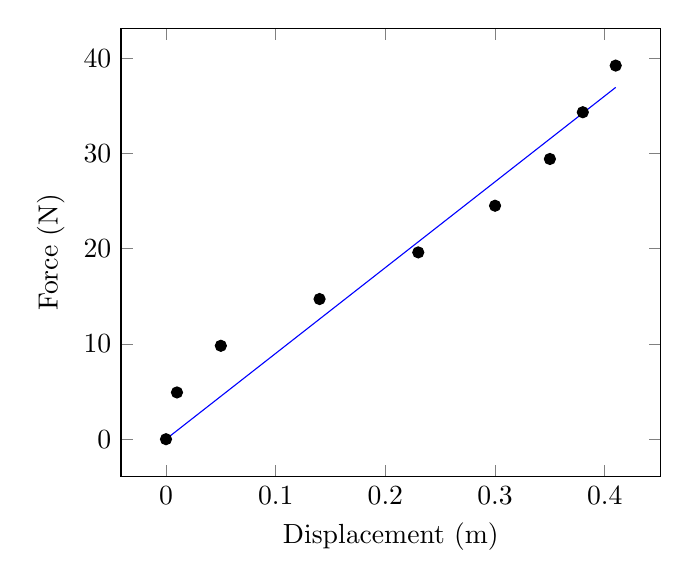
\begin{tikzpicture}
	\begin{axis}[xlabel=Displacement $(\si{\meter})$,
				 ylabel=Force $(\si{\newton})$]
	
	\addplot[only marks] coordinates {
		(0.00, 0.00)
		(0.01, 4.91)
		(0.05, 9.81)
		(0.14, 14.72)
		(0.23, 19.62)
		(0.30, 24.52)
		(0.35, 29.43)
		(0.38, 34.34)
		(0.41, 39.24)
	};
	
	\addplot[no marks, blue, domain=0:0.41] {90.12*x};
	
	\end{axis}
	\end{tikzpicture}
	\caption{text}
\end{figure}



\section{Discussion}

\section{Conclusion}

\bibliography{my_bib}
\bibliographystyle{ieeetr}

\end{document}